\section{Type Checker}
\subsection{Parsing and Lexing}
The parser and lexer upon which the type checker has been built is based on the textual \textsc{bon} lexer and parser created by Joseph Kiniry for the Extended \textsc{bon} Tool Suite \cite{ebon} (henceforth denoted \textsc{ebon}). At the outset of this project, the rule part of the parser was already finished (although some minor alterations were made to it to fit the implementation of the type checker), while the semantic actions were partially implemented. The implementation of these actions have now been completed. No alterations were made to the lexer.
\paragraph{} The parser generating the abstract syntax tree is a tree parser, creating a model object graph of textual \textsc{bon} elements (or a parse error) as a result. Like the parser, these model classes were also partially implemented initially, but have now been completed.

%Add paragraph with a more design-oriented view on the parser

\paragraph{} The parser and lexer used for the type checker has been done using the \textit{Gobo} tools \textit{gelex} and \textit{geyacc} \cite{gobo}.
\subsubsection{Deviations from the Grammar}
The grammar for the parser deviates from the grammar in \cite{walden1995} in a few places. Most of these were already present in the \textsc{ebon} grammar file.
%Result token
\paragraph{} A \textit{Result} token was added for use in feature contracts in formal specifications. It represents the resulting value of its enclosing feature, just like its Eiffel counterpart.
%Expressions
\paragraph{} In order to be able to express the grammar in a proper type hierarchy, some alterations regarding the formal assertions were made. In particular, the original grammar implies the following relationship \cite[p.~357]{walden1995}:
\begin{center}
\textit{Expression} \textless : \textit{Operator\textunderscore expression} \textless : \textit{Parenthesized} \textless : \textit{Expression}
\end{center}
As this situation cannot be modeled due to circular inheritance, a \textit{Parenthesized} element is treated as a boolean expression instead of an operator expression. Changes have been made to \textit{Set\textunderscore expression} accordingly, as it refers to \textit{Operator\textunderscore expression}.
%Named indirection - indirection lists
\paragraph{} The class name in a named indirection has been made optional in order to allow for situations such as the one described in \cite[p.~372]{walden1995}, example in figure B.9. Contrary to the \textsc{ebon} grammar, the indirection list has not been made optional, as this would create ambiguity between a formal generic name and a named indirection; when confronted with a generic indirection, the parser needs to be able to disambiguate between these.

\subsection{Design Decisions}
This section discusses the overall design decisions of the textual \textsc{bon} type checker, both with regards to the high-level structure of the system and the more low-level implications of specifying the underspecified grammar.
\subsubsection{Type Checking Patterns}
When discussing the overall structure and design of the type checker, two patterns were considered; the visitor pattern, and a procedural pattern inspired by a more functional approach.
\subsubsubsection{The Visitor Pattern} %The visitor pattern
The visitor pattern provides a way to add a new feature to a hierarchy of classes without having to implement the feature in the class itself \cite{martin2002}. Instead, the functionality is implemented in a feature in a visitor class, the content of which is unknown to the visited object. The main idea of the pattern is the technique called \textit{dual dispatch}, called as such due to the two polymorphic dispatches happening when executing the visitor: 
\begin{figure}[H]
    \scalebox{0.7}{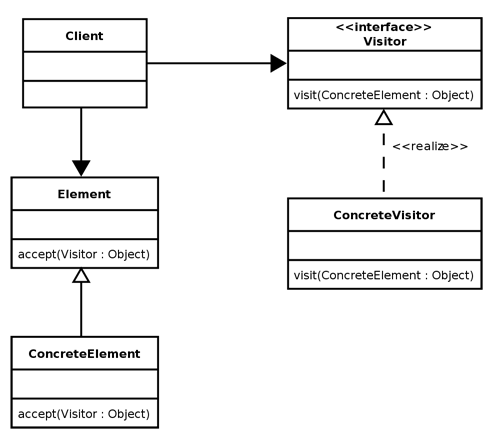
\includegraphics{images/Visitor.png}}
    \caption[Visitor pattern]{Visitor pattern (source: http://en.wikipedia.org/wiki/Visitor\textunderscore pattern)}
    \label{fig:visitor-pattern}
\end{figure}
\begin{enumerate}
\item Each concrete class in the hierarchy must have an \textit{accept} feature that accepts a general (often deferred) visitor type as its argument, as depicted in figure \ref{fig:visitor-pattern}, and the first dispatch resolves the general visitor type into a concrete visitor,
\item The actual feature called on the concrete visitor is determined (via overloading) by the input type passed to the \textit{visit} feature of the visitor, which is resolved by the second dispatch.  
\end{enumerate}
In the above, it is implied that the concrete visitor class has an implemented \textit{visit} feature for each of the types in the hierarchy that is to be visited. Since feature overloading is not supported in Eiffel, the second dispatch would be implemented by a visit feature with a unique name for each of the types in the hierarchy.
%\paragraph{} -- MIGHT NOT BE INCLUDED AT ALL
% REWRITE PRACTICAL IMPLICATIONS
%The practical implications of implementing the visitor pattern would be the creation of a class \textsc{type}\textunderscore\textsc{checking}\textunderscore\textsc{visitor} with visit features for each textual \textsc{bon} element, for instance \textit{visit}\textunderscore\textit{class}\textunderscore\textit{chart}. In turn, the class \textsc{class}\textunderscore\textsc{chart} would have a feature \textit{visit} (\textit{visitor:}  \textsc{visitor}), where the visitor for type checking is a subtype of \textsc{visitor}.
%\begin{centering}
%\textit{accept}: \textsc{visitor} $\rightarrow$ ()\\
%\textit{visit}\textunderscore\textit{bon}\textunderscore\textit{element}: \textsc{bon}\textunderscore\textsc{element} $\rightarrow$  ()\\
%\end{centering}
\subsubsubsection{The Procedural Approach} %The procedural pattern
The more procedural approach is inspired by the visitor pattern, but differs from it in an important aspect. In this approach, type checking is done by defining a feature of the following form for each \textsc{bon} element:
\begin{center}
\textit{type}\textunderscore\textit{check}\textunderscore\textit{bon}\textunderscore\textit{element}: \textsc{bon}\textunderscore\textsc{element} $\rightarrow$  \textsc{boolean}\\
\end{center}
Each of these features takes a \textsc{bon} element as argument and produces a \textsc{true} or \textsc{false} answer, depending on the semantic correctness of the input. Like the visitor pattern, a type checking feature is implemented for each of the elements in class hierarchy; but unlike the visitor pattern, the feature is called as a function on the \textsc{bon} element, evaluating whether or not the element is well-typed, instead of ''asking'' the element itself whether it is well-typed.
\subsubsubsection{Choosing a Pattern}
%We don't have to implement a visit feature in all the MOG classes.
%Context argument
In both approaches, all of the type checking code is placed in a single class. The great benefit of the visitor pattern is its generality and object-oriented nature. But this comes at a cost. For the \textit{accept} feature to be sufficiently general, it cannot return a specific type, and consequently the information about the well-typedness of an element must be saved in the state of the visitor. Accordingly, the object-oriented nature of the visitor pattern means that the \textit{accept} feature would have to be implemented in every class of the model object graph, only to redirect the call back to the visitor.
\paragraph{} The functional nature of the procedural approach means that information about the well-typedness of an element can be propagated through the type checker as results of feature calls. Also, as the type checker is called as a function on an element, and not on the element itself, no additions have to be made to the classes of the model object graph. But this also means a loss of generality, which is the main drawback of this approach; no interface is provided for easy traversal of the object graph for reasons other than type checking.
\paragraph{} For the structure of the type checker, the procedural approach has been chosen, as the lack of generality seems acceptable when compared to the drawbacks of the visitor pattern. The added generality of the visitor pattern does not justify the extra overhead it would impose on the implementation of the type checker.

\subsubsection	{Phases of the Type Checker}
\label{design-phases}
As suggested by Appel and Palsberg in \cite[section~5.2]{appel2004} for type checking MiniJava, type checking of textual \textsc{bon} also happens in two phases. Just as for MiniJava, this is done because classes and clusters in textual \textsc{bon} are mutually recursive\footnote{This is not entirely precise as a class does not rely on a cluster to be correct.}.
\subsubsubsection{The First Phase}
During the first phase, the context is built; i.e. the type checker stores information about all defined elements in the AST in appropriate data structures. Informally, the first phase answers the question: ''What do we know?''. An element is considered to be defined when a specification for it appears in the AST. For instance, a class in a formal specification is defined when a class specification for it exists. If the class is merely mentioned in an inheritance clause of another class or in a cluster, it is not defined.
\paragraph{} To avoid the rather substantial amount of symbol tables hinted at in \cite{appel2004} (e.g. mapping from classes to features, from features to type, from features to arguments etc.), the aforementioned 'appriopriate data structures' is made as a class hierarchy, in which a \textsc{bon} class is represented by a context class with references to features, ancestors, generics, and so forth. These will be explained in greater in detail in section \ref{implementation-context-class-structure}.
\subsubsubsection{The Second Phase}
During the second phase, the relationships between the defined elements are checked. Most of the actual type checking happens in this phase, as only a few rules can be checked without knowledge of the entire context. Specifically, if a type checking feature for an element returns \textsc{true} in the second phase, then the element in question is well-typed. If the opposite is the case, an error message is emitted and \textsc{false} is returned. In practice, not all rules can be checked in the second phase, e.g. checking for circular inheritance, as they depend on the correctness of the relationships between the defined elements. Details about the handling of these rules are explained in section \ref{implementation-unresolved-elements}

\subsubsection {Type System}
\label{design-type-system}
Textual \textsc{bon} as defined in \cite{walden1995} is quite underspecified in several key points, most likely to preserve flexibility of the notation (i.e. to avoid tight coupling to a single or a few programming languages). This section presents the necessary specifications and delineations made in order to type check the notation.
\subsubsubsection{Names}
\label{design-type-names}
All names of classes and clusters must be unique. There is no notion of a fully qualified name, and as such, even if static references with cluster qualification are used, it is not possible to have two classes or clusters with identical names.
\paragraph{} In the current implementation of the type checker, there is no relation or information sharing between the type contexts of informal and formal specifications, respectively. Consequently, it is possible for a class or cluster in an informal specification to have a name identical to a class or cluster in a formal specification.
\subsubsubsection{Informal Structure}
Following the example set forth in \textsc{bon}c \cite{bonc}, a class in an informal \textsc{bon} specification must be in exactly one cluster. Similarly, a cluster in an informal specification must appear in a system chart or be a subcluster of a cluster that appears in a system chart.
\subsubsubsection{Formal Structure}
Unlike the structure of informal specifications, a class does not have to be specified in a cluster specification in a formal specification (there is no equivalent to system charts for formal specifications). As one might wish to describe a part of the system at a more granular level in a static diagram than one would do in an informal specification, it is not required that the entire system structure is specified for the specification to type check. If static references with cluster qualifications are used, however, the type checker requires that the cluster relations implied by the static references are explicitly defined.
\subsubsubsection{Variance}
When type checking features and feature arguments, the legal types of variance has to be implemented in the type checker in order to determine the well-typedness of these elements. Seeing as Eiffel implements covariance for both feature types and feature argument types  \cite[the~Covariance~rule]{meyer2001}, the same is supported in the type checker for feature types and feature argument types in formal specifications of textual \textsc{bon}. This is mainly due to the fact that the primary objective of the textual \textsc{bon} type checker is to type check specifications extracted from Eiffel source code in EiffelStudio.
\paragraph{} However, in a future version of the type checker, it might be desirable to be able to customize the legal types of variance during type checking, in order to consistently type check bon specifications extracted from other programming languages than Eiffel. This is left as an option for further development, and is not prohibited by the current design of the type checker.
\subsubsubsection{Inheritance}
As specified in \cite[p.~65]{walden1995}, single, multiple, and repeated inheritance are all allowed. Circular inheritance (a class inheriting from itself) is not allowed, though, and is enforced by the type checker. Conformance between generic types is not considered; thus, there is no conformance between \textsc{list}[\textsc{integer}] and \textsc{list}[\textsc{real}], even though \textsc{integer} inherits from \textsc{real}.
\subsubsubsection{Assertions}
Due to the non-restrictive nature of the assertion grammar presented in \cite{walden1995}, some restrictions have to be made in order for the assertion grammar to type check.
\paragraph{} Firstly, the original grammar allows for a restriction or a proposition in a quantification to be a constant, calls, or operator expression of arbitrary type. The type checker enforces these to have boolean type; the definition of boolean type in this respect is defined in section \ref{implementation-def-boolean-type}.
\paragraph{} Secondly,  the grammar defines a set expression to be an operator expression or a call of arbitrary type, or an enumerated set with elements of possibly unrelated types. To type check a set expression, the type checker enforces it to be an expression of an enumerable type (no matter if it is an operator expression or a call), or to be an enumerated set in which all of the elements conform to at least one of the elements in the set. Implementation details of these restrictions are presented in section \ref{implementation-set-expressions}.



